\begin{Example}[icu2]{Survival in the ICU}
The four variable model from \exref{ex:icu1} predicting survival in the ICU
was examined for influential cases with the \macro{INFLOGIS}.
The following macro call produces an influence plot of the \pname{DIFCHISQ}
statistic against hat values, shown in \figref{fig:icu12}.
\begin{listing}
%inflogis(data=icu, y=died, x=age cancer uncons admit,
   id=id,
   gy=difchisq,
   gx=hat);
\end{listing}

%% one figure
\begin{figure}[htb]
  \centering
  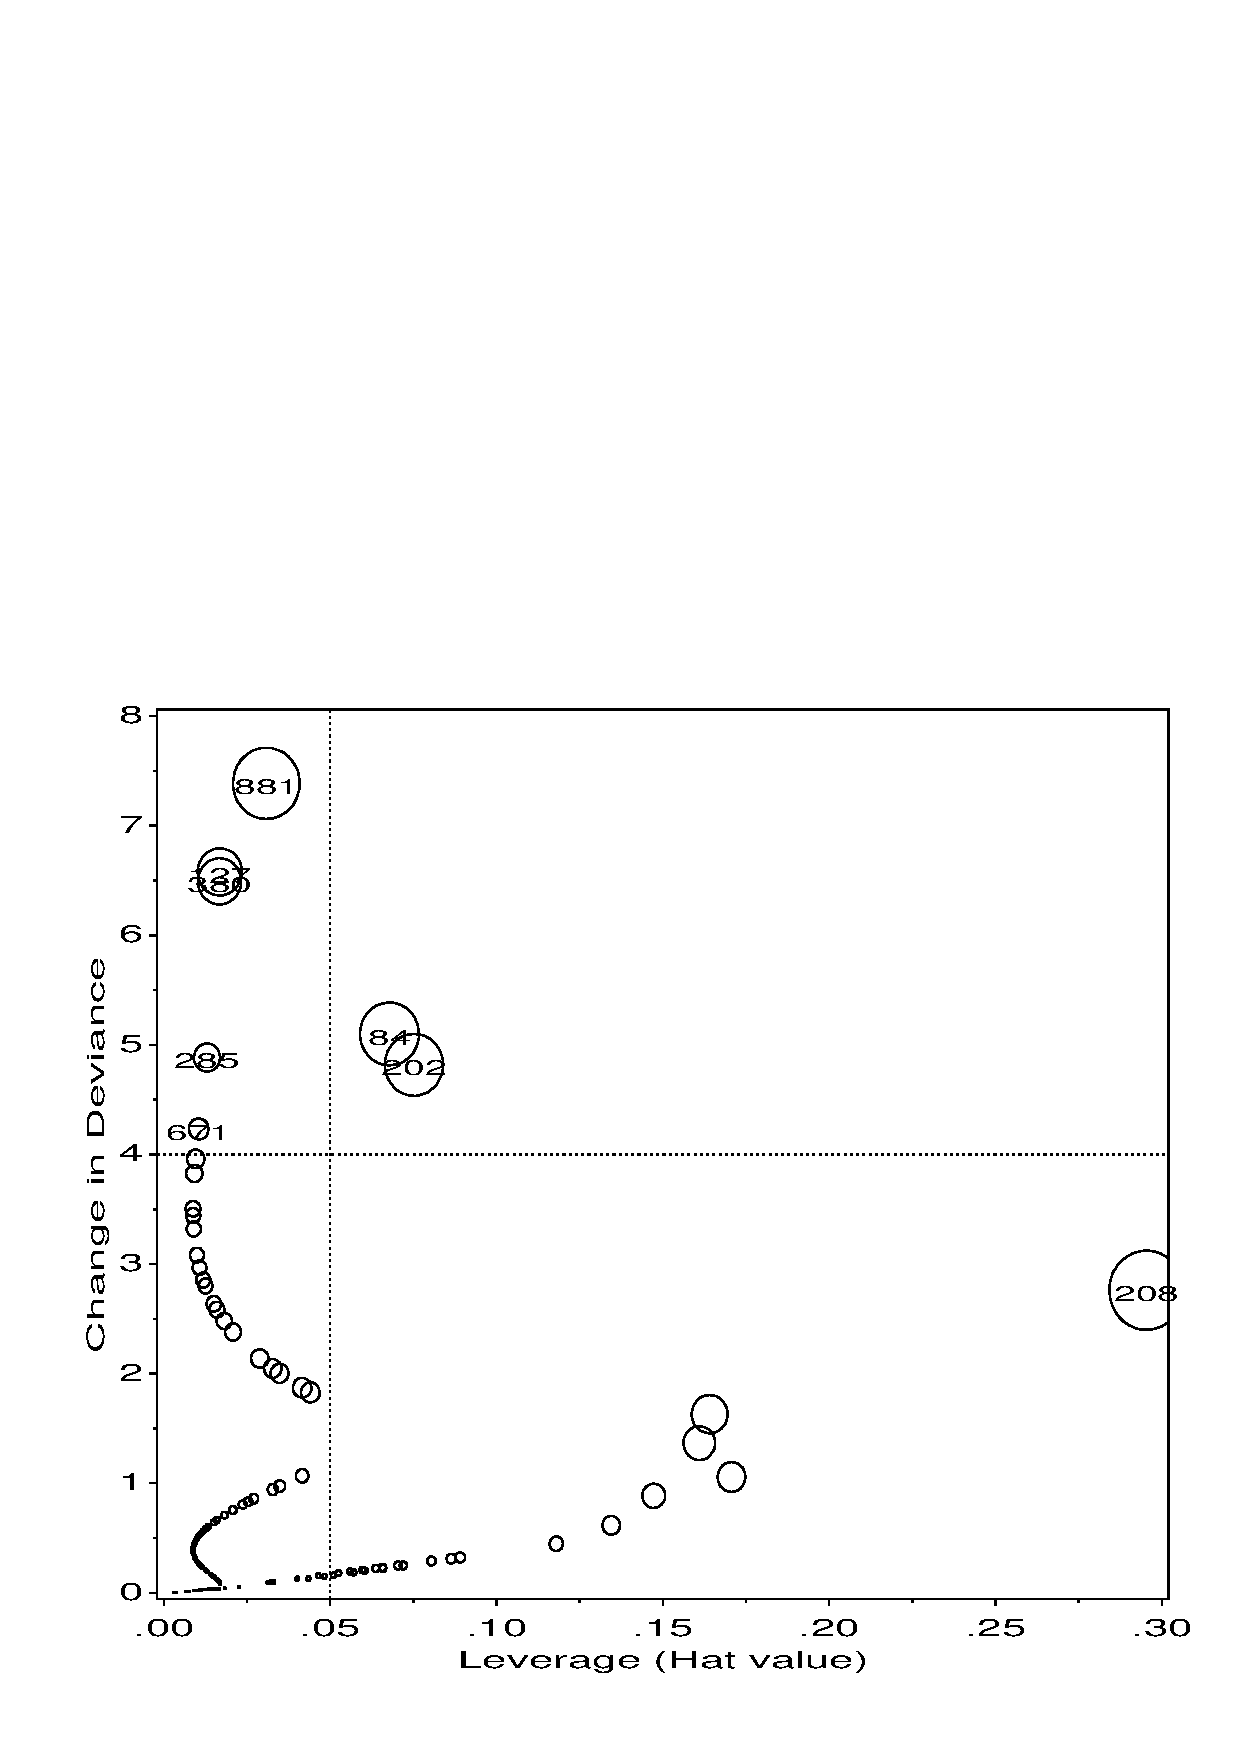
\includegraphics[scale=.6]{ch6/fig/icu12}
  \caption[ICU Survival data: Influence plot]{ICU Survival data: Influence plot}%
  \label{fig:icu12}
\end{figure}

Details for the cases identified in the figure are shown in \outref{out:icu1.2}.
None of the cases are particularly influential on the model coefficients overall:
the largest $C_i$ is only 1.04.
Case 208, with the largest hat value, is unusual on the predictors
in this sample: a 70 year old man without cancer, admitted on an elective
basis (who nonetheless died).
On the other hand, case 881, an 89 year old male, admitted unconscious
as an emergency case is poorly predicted because he survived.
Similarly, two other cases (127, 380) with large $\Delta \chi_{(-i)}^2$
are poorly predicted because they died, although they were
young, did not have cancer, and conscious at admission.
From this evidence we might conclude that none of these cases greatly affects the model, its coefficients,
or interpretation.
\begin{Output}[htb]
\caption{ICU data: Influential cases}\label{out:icu1.2}
\small
\verbatiminput{ch6/out/icu1.2}
\end{Output}

That conclusion might not be warranted without further study, particularly
in terms of influence on individual coefficients.
The DFBETAs \eqref{eq:dfbeta} may be obtained in an \ODS\ as shown below:
\begin{listing}
proc logistic data=icu;
   model died = age admit cancer uncons;
   output out=stats dfbetas=dbint dbage dbadmit dbcancer dbuncons ;
\end{listing}

%% two subfig side-by-side
\begin{figure}[htb]
 \begin{minipage}[t]{.49\linewidth}
  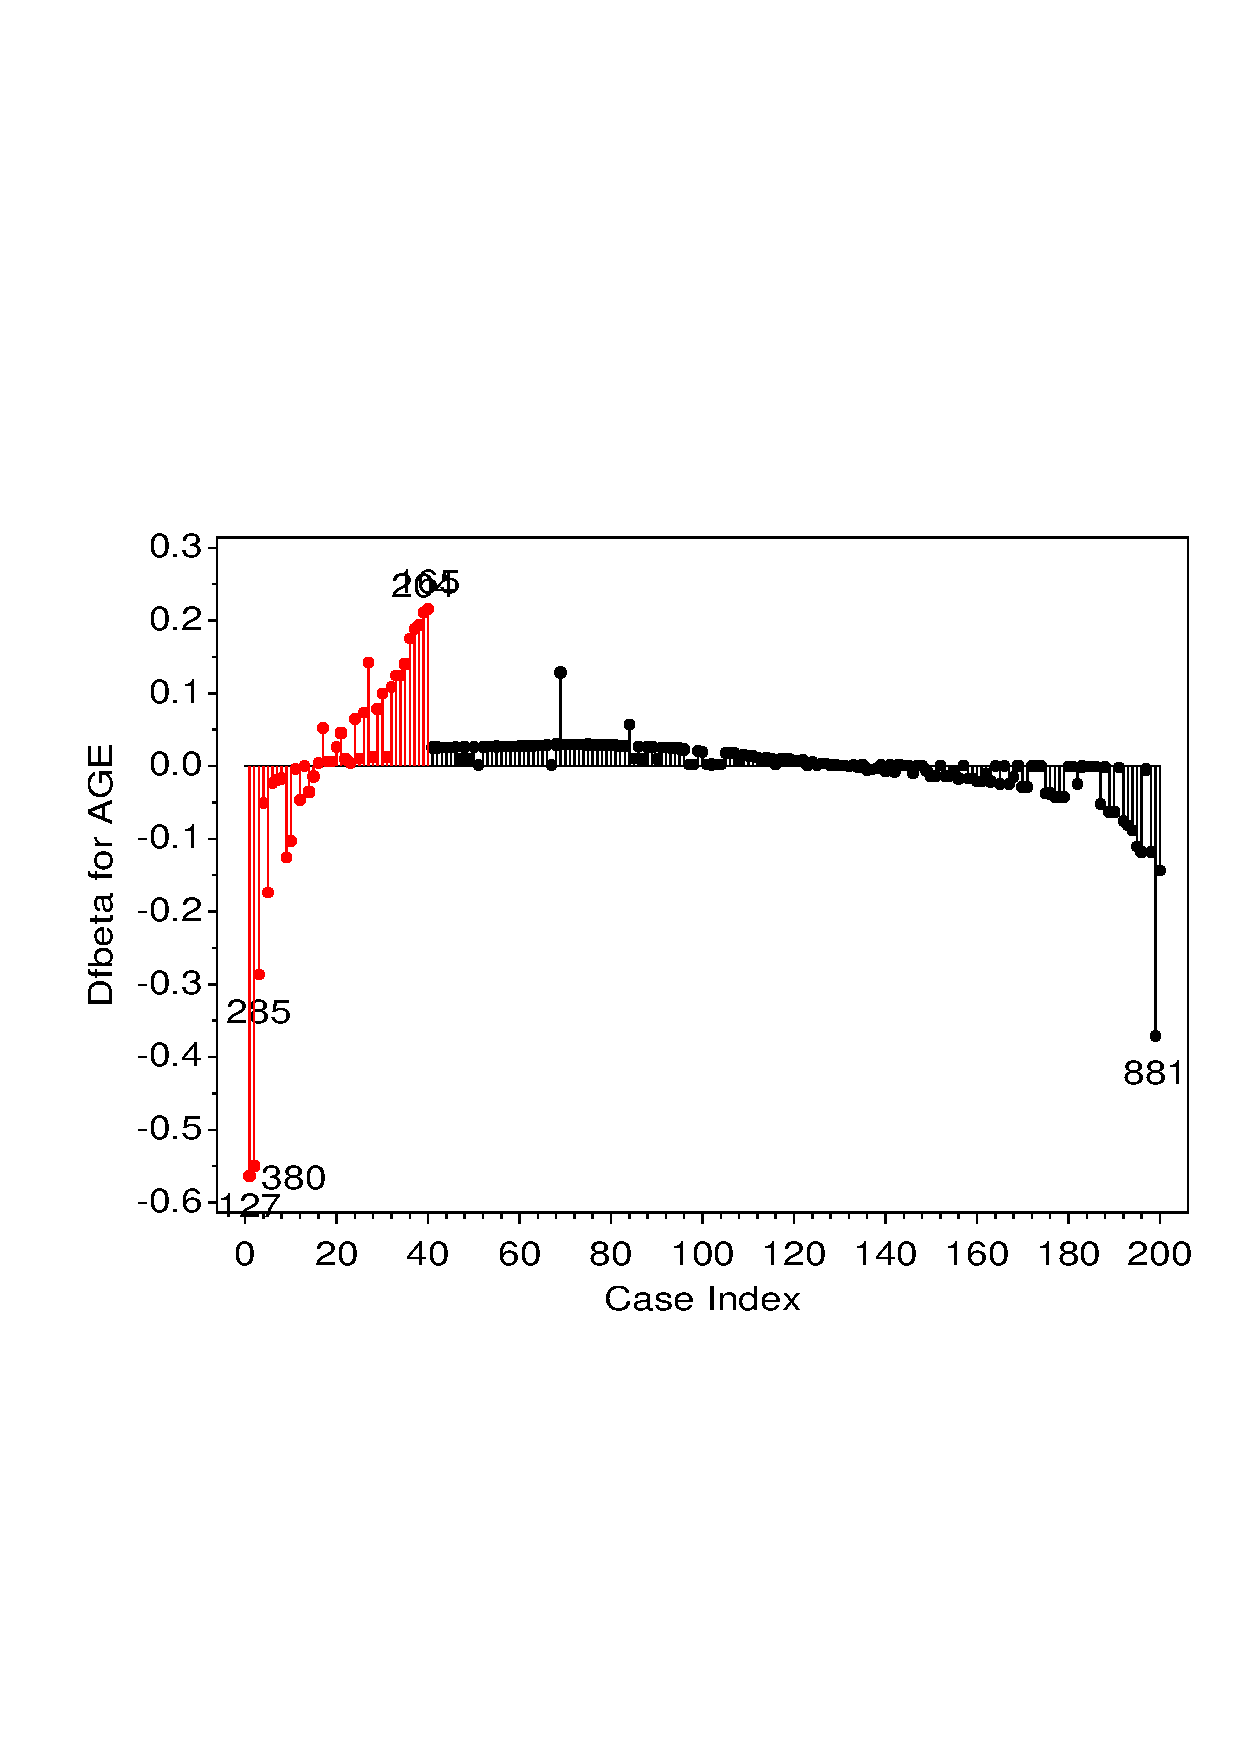
\includegraphics[width=1\linewidth,clip]{ch6/fig/icu4b1}
 \end{minipage}%
 \hfill
 \begin{minipage}[t]{.49\linewidth}
  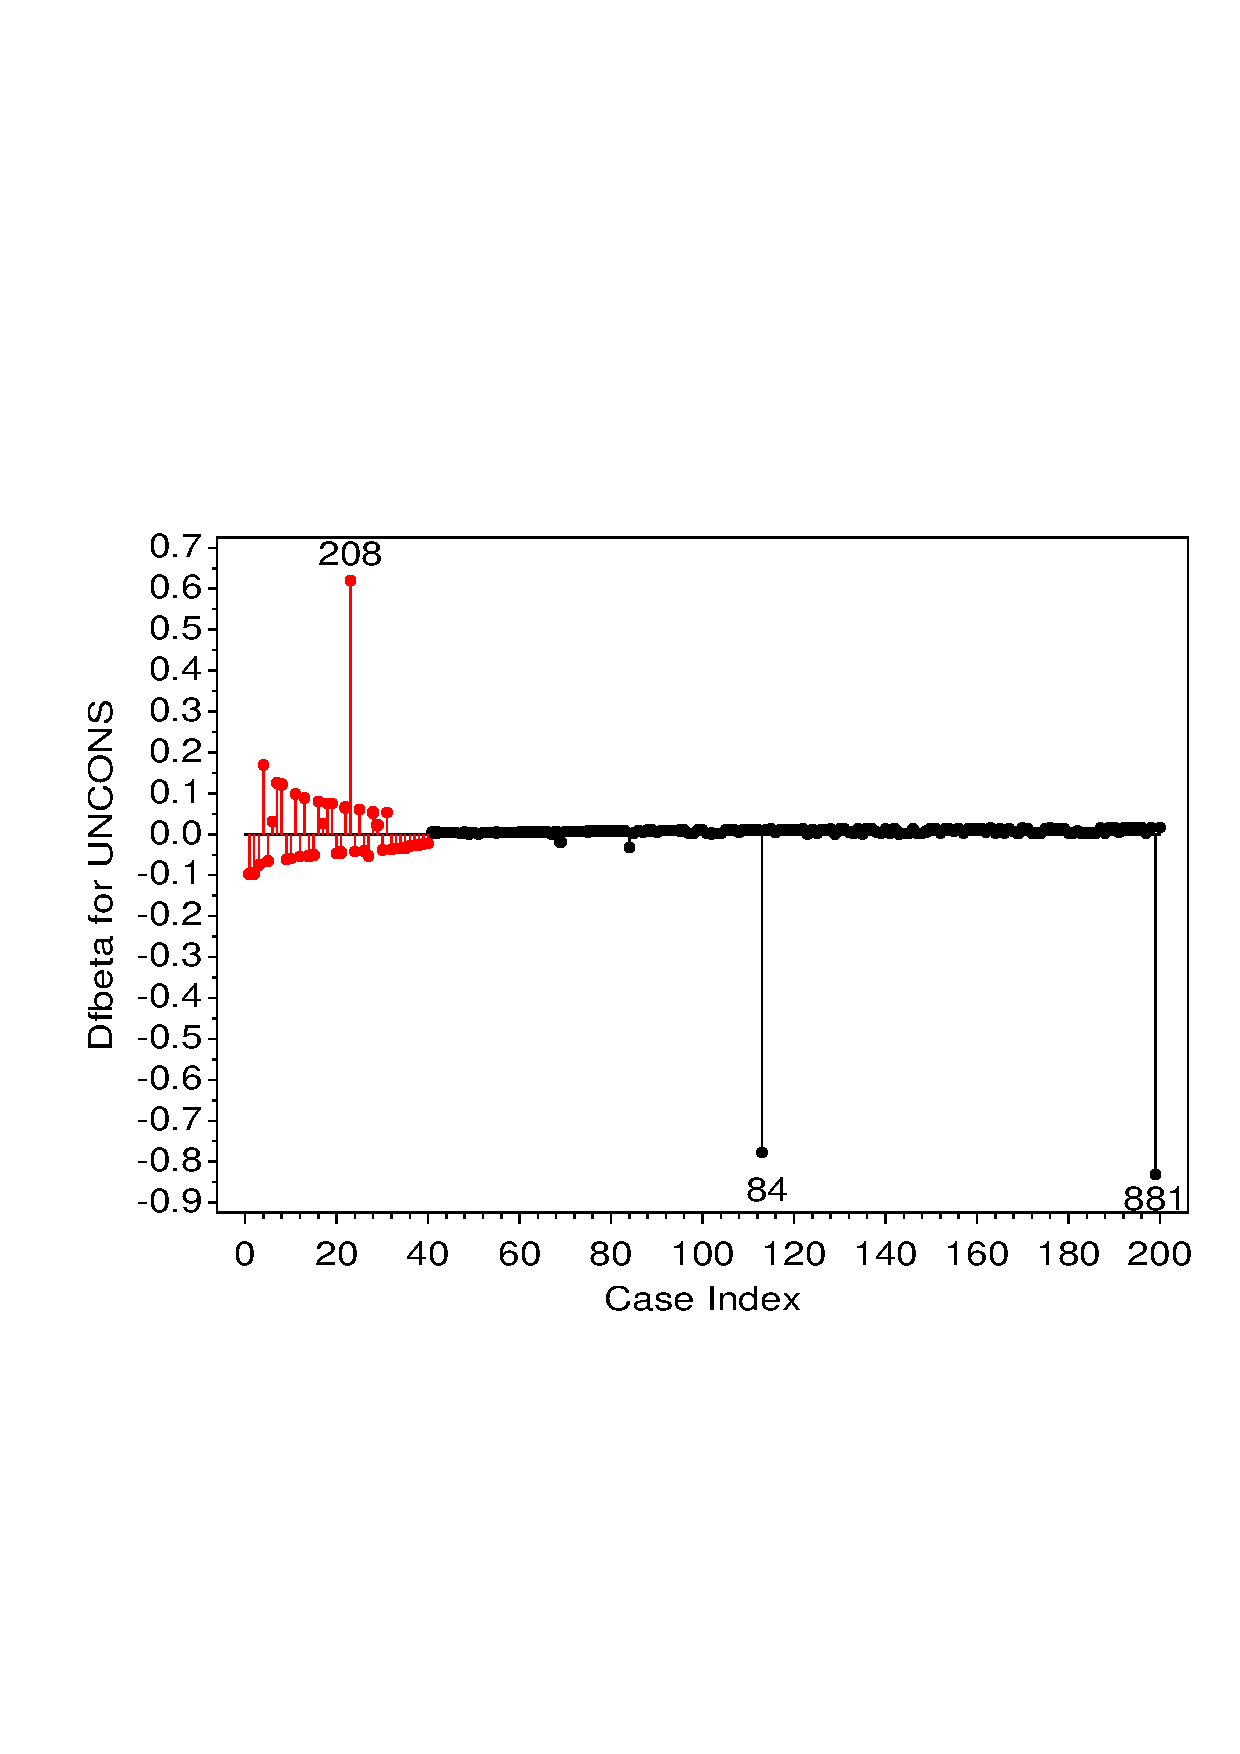
\includegraphics[width=1\linewidth,clip]{ch6/fig/icu4b2}
 \end{minipage}
 \caption{ICU data: DFBETA index plots for Age and Uncons}\label{fig:icu4b}
\end{figure}
Individual DFBETAs are often graphed as \emph{index plots}, that is,
for variable $j$ a plot of DFBETA$(i, j)$ against the case index $i$.
In such plots, it is helpful to label points with large absolute
values when (as here) the case number is not meaningful.
For example, the following statements produce an index plot of the
DFBETA for age, shown in \figref{fig:icu4b}.
The \macro{LABEL} is used to label points by the patient \pname{id},
where the DFBETA value exceeds 0.2 (an arbitrary value) in magnitude.
\begin{listing}
data stats;
   set stats;
   case = _n_;

%label(data=stats, x=case, y=dbage, text=put(id,3.), pos=-,
    subset=abs(dbage)>.2, out=labs);

proc gplot data=stats;
   plot dbage * case = died /
      anno=labs frame nolegend vaxis=axis1 haxis=axis2 vm=1;
   symbol1 i=needle v=dot c=black;
   symbol2 i=needle v=dot c=red;
   axis1 label=(a=90) length=4.5in;
   axis2 offset=(2) ;
\end{listing}
An alternative display, which is often more informative (though possibly more complex) is a scatterplot matrix of the DFBETAs, perhaps with other
influence diagnostics as well.
The pairwise scatterplots help to highlight observations which are
influential on both or only one of each pair of measures.
An example is shown in \figref{fig:icu4a}, produced with the
\macro{SCATMAT}:
\begin{listing}
%scatmat(data=stats,
   var= dbAge dbAdmit dbCancer dbUncons, group=died,
   symbols=star square,
   plotopt=%str(href=-0.2 0.2 vref=-0.2 0.2 cvref=graya0 chref=graya0));
\end{listing}

%% one figure
\begin{figure}[htb]
  \centering
  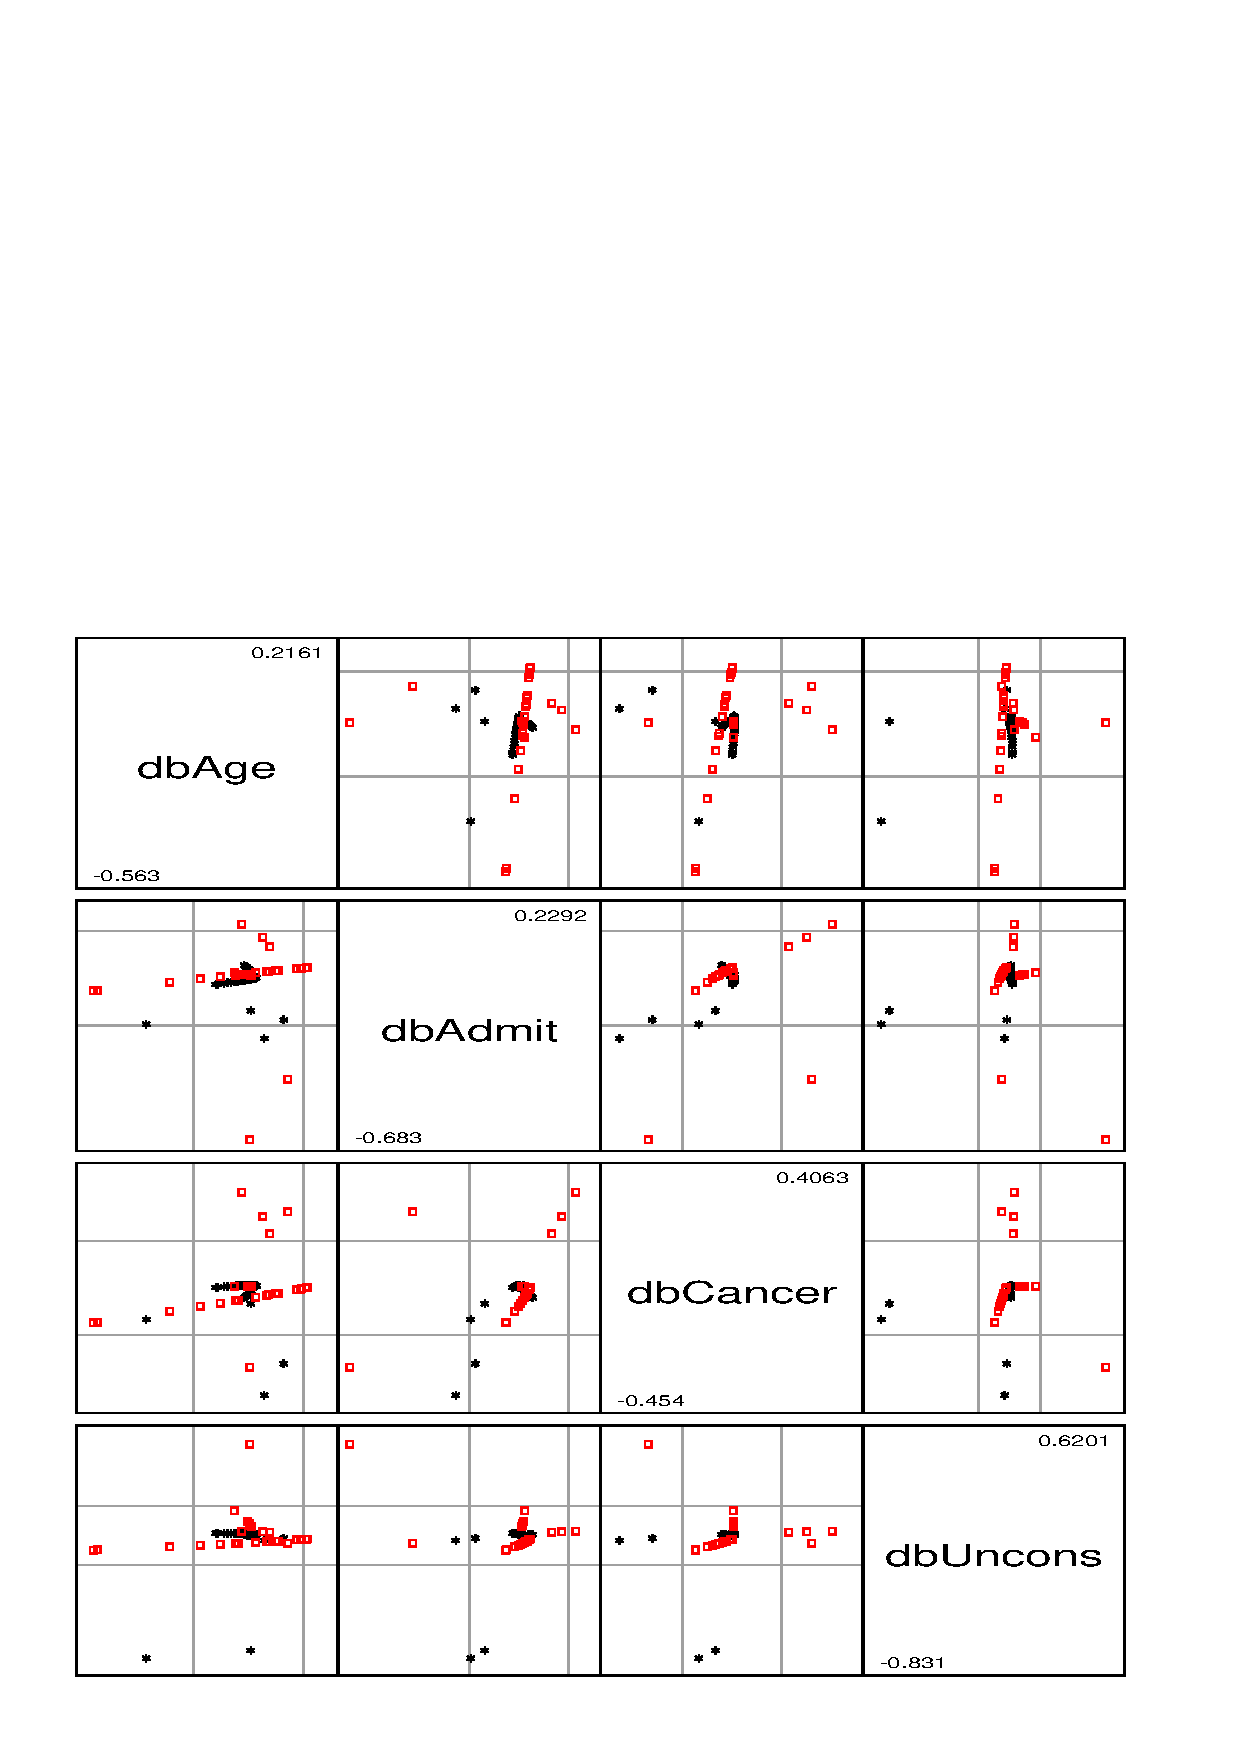
\includegraphics[scale=.75]{ch6/fig/icu4a}
  \caption[ICU Survival data: Scatterplot matrix of DFBETAs]{ICU Survival data: Scatterplot matrix of DFBETAs.  Those who lived are shown by $\star$s,  those who died are shown by squares.
  The reference lines indicate values of $\pm 0.2$ on each statistic.}%
  \label{fig:icu4a}
\end{figure}
Most of the observations are in the central rectangle, corresponding to
small values ($< \pm 0.2$) on both measures, but several points stand out
on the pairwise combinations.  For example, the bottom row and
rightmost column (DFBETA for \pname{UNCONS})
highlight two observations for patients who lived ($\star$s)
whose omission would decrease the coefficient for \pname{UNCONS}
considerably, and one who died whose omission would increase it.
Other observations outside the central rectangle might also be investigated.
\end{Example}
